\chapter{Methodology} \label{sec-methodology}

This chapter describes the methodology used in this work. It is organized as follows: Section \ref{sec-defining-problem} defines the problem to be solved, Section \ref{sec-vel-mass-correction} describes the simulation parameters for the velocity and mass correction and Section \ref{sec-ml-model} describes the machine learning model that will be used to reconstruct the track irregularities.

\section{Defining the Problem} \label{sec-defining-problem}

In this dissertation, the main objective is to develop a unsupervised machine learning model that can reconstruct track irregularities from acceleration data. The reconstructed profiles can be then compared to the standard limits to support maintenance planning, or, in the case of an off limits irregularity, a defect can be identified and repaired before it causes an issue. 

Figure \ref{fig:flowchart} shows a flowchart of the step-by-step methodology that will be used to achieve this goal. 

To acquire data, a multibody simulation will be set up in the software SIMPACK with the support of the dynamic simulation team, as the implementation details of the model are not the focus of this thesis. The simulation model will first be validated using real data from a section of track geometry measured by the TCG and the corresponding acceleration measurements collected by the IRV. The simulated wagon will replicate the IRV sensor configuration, described in detail in Pires et al. \cite{PIRES2024107191}, measuring the vertical acceleration on the side frames, the displacement of the secondary suspension, and the triaxial carbody acceleration. Once validated, the simulation will be used to generate a dataset containing sensor data for different track irregularities, velocities, and wagon masses. This search space will be explained in more detail in Section \ref{sec-vel-effect-measurement}.

With this dataset, a study will be conducted to analyze the effect of the wagon mass and velocity on the acceleration measurements. The goal is to understand how these parameters affect the data and develop a correction method, using similar approaches described in Sections \ref{sec-vel-effect-measurement} and \ref{sec-mass-effect-measurement}, to correct the acceleration data.

The corrected acceleration data will then be used to train a machine learning model for reconstructing track irregularities. Model performance will be evaluated using real-world data. Finally, a threshold will be defined on the reconstructed profiles to determine when maintenance is required, enabling condition-based planning based solely on acceleration measurements.

\begin{figure}[H]
    \centering
    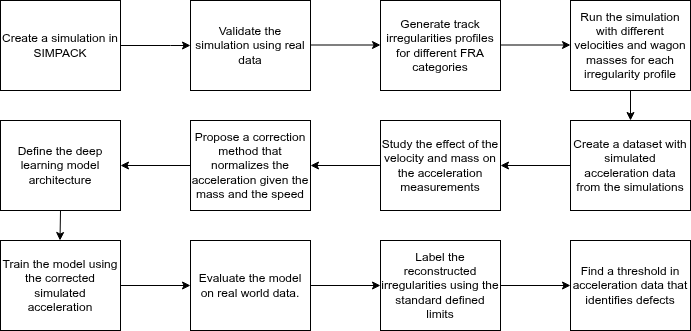
\includegraphics[width=16cm]{Cap3_Methodology/Flowchart/Flowchart.png}
    \caption{Flowchart of the proposed methodology.}
    \label{fig:flowchart}
\end{figure}

\section{Search Space of the SIMPACK Simulation} \label{sec-vel-mass-correction}

As stated in Section \ref{sec-defining-problem} a SIMPACK simulation will run across a search space composed of different velocities, wagon masses and track irregularities. Table \ref{table:search_space} summarizes the parameter ranges. Each simulation will test one combination until all possibilities have been explored.

\begin{table}[H]
\centering
\begin{tabular}{l l}
\hline
\textbf{Parameter} & \textbf{Values} \\
\hline
Velocity (km/h) & 5, 10, 15, 20, 25, 30, 35, 40, 45, 50, 55, 60, 65 \\
Wagon mass (tons) & 0, 51, 102 \\
Track irregularity & No irregularities, FRA 6, FRA 5, FRA 4, Real Irregularities \\
\hline
\end{tabular}
\caption{Search space for the SIMPACK simulation.}
\label{table:search_space}
\end{table}

The velocity range was defined to cover the typical train velocity operation in the Brazilian Estrada de Ferro Vitória a Minas (EFVM) railway. Wagon masses corresponds to the unloaded wagon class, the half loaded wagon and the fully loaded wagon class. The track irregularities were defined to cover a good track condition (FRA 6), a regular condition track (FRA 5) and a not so good condition track (FRA 4). The "real irregularities" corresponds to a measured track geometry that contains some defects, such as a switch and some misalignments. The "no irregularities" serves as a baseline case to the study.

From this generated data, an approach similar to Balouchi, Bevan and Formston \cite{Balouchi02092021} will be used to correct the measurements. In this method, a linear or quadratic regression model will be fitted to the absolute maximum acceleration data across different velocities and different wagon masses. The goal is to develop a correction method that is independent from the track irregularity. The final regression model will be evaluated on real world data.

\section{Machine Learning Model} \label{sec-ml-model}

The machine learning model to be used in this thesis needs to satisfy a set of requirements. These requirements are:
\begin{itemize}
    \item The model can not depend on labels, i.e., it needs to be an unsupervised model;
    \item The model should consider input data as being sequential, i.e., it needs to take into consideration temporal correlations;
    \item The model needs to be able to handle noisy data;
    \item The model should be able to be trained on simulated data and perform well on real world data without the need of retraining.
\end{itemize}

Based on these requirements, the chosen approach is to use a deep learning model that utilizes the methods described in Section \ref{sec-model-basics}, as it is the most robust approach for handling complex data. These outputs of this model will be then compared to the geometric limits in the Brazilian standard to develop a threshold for maintenance planning based on acceleration data.
